\documentclass[a4paper]{article}
\usepackage{tikz}
\usepackage{geometry}
\usepackage{graphicx}
\usepackage{natbib}
\usepackage{amsmath}
\usepackage{amssymb}
\usepackage{amsthm}
\usepackage{paralist}
\usepackage{epstopdf}
\usepackage{tabularx}
\usepackage{longtable}
\usepackage{multirow}
\usepackage{multicol}
\usepackage[hidelinks]{hyperref}
\usepackage{fancyvrb}
\usepackage{algorithm}
\usepackage{algorithmic}
\usepackage{float}
\usepackage{paralist}
%\usepackage[svgname]{xcolor}
\usepackage{enumerate}
\usepackage{array}
\usepackage{times}
\usepackage{url}
\usepackage{fancyhdr}
\usepackage{comment}
\usepackage{environ}
\usepackage{times}
\usepackage{textcomp}
\usepackage{caption}
\usepackage{bbm}


\urlstyle{rm}

\setlength\parindent{0pt} % Removes all indentation from paragraphs
\theoremstyle{definition}
\newtheorem{definition}{Definition}[]
\newtheorem{conjecture}{Conjecture}[]
\newtheorem{example}{Example}[]
\newtheorem{theorem}{Theorem}[]
\newtheorem{lemma}{Lemma}
\newtheorem{proposition}{Proposition}
\newtheorem{corollary}{Corollary}

\floatname{algorithm}{Procedure}
\renewcommand{\algorithmicrequire}{\textbf{Input:}}
\renewcommand{\algorithmicensure}{\textbf{Output:}}
\newcommand{\abs}[1]{\lvert#1\rvert}
\newcommand{\norm}[1]{\lVert#1\rVert}
\newcommand{\RR}{\mathbb{R}}
\newcommand{\CC}{\mathbb{C}}
\newcommand{\Nat}{\mathbb{N}}
\newcommand{\br}[1]{\{#1\}}
\DeclareMathOperator*{\argmin}{arg\,min}
\DeclareMathOperator*{\argmax}{arg\,max}
\renewcommand{\qedsymbol}{$\blacksquare$}

\definecolor{dkgreen}{rgb}{0,0.6,0}
\definecolor{gray}{rgb}{0.5,0.5,0.5}
\definecolor{mauve}{rgb}{0.58,0,0.82}

\definecolor{C0}{HTML}{1F77B4}
\definecolor{C1}{HTML}{FF7F0E}
\definecolor{C2}{HTML}{2ca02c}
\definecolor{C3}{HTML}{d62728}
\definecolor{C4}{HTML}{9467bd}
\definecolor{C5}{HTML}{8c564b}
\definecolor{C6}{HTML}{e377c2}
\definecolor{C7}{HTML}{7F7F7F}
\definecolor{C8}{HTML}{bcbd22}
\definecolor{C9}{HTML}{17BECF}

\newcommand{\Var}{\mathrm{Var}}
\newcommand{\Cov}{\mathrm{Cov}}
\newcommand{\sgn}{\mathrm{sgn}}

\newcommand{\vc}[1]{\boldsymbol{#1}}
\newcommand{\xv}{\vc{x}}
\newcommand{\Sigmav}{\vc{\Sigma}}
\newcommand{\alphav}{\vc{\alpha}}
\newcommand{\muv}{\vc{\mu}}

\newcommand{\red}[1]{\textcolor{red}{#1}}

\def\x{\mathbf x}
\def\y{\mathbf y}
\def\w{\mathbf w}
\def\v{\mathbf v}
\def\E{\mathbb E}
\def\R{\mathbb R}
\def\V{\mathbb V}
\def\ind{\mathbbm 1}

% TO SHOW SOLUTIONS, include following (else comment out):
\newenvironment{soln}{
	\leavevmode\color{blue}\ignorespaces
}{}


\hypersetup{
	%    colorlinks,
	linkcolor={red!50!black},
	citecolor={blue!50!black},
	urlcolor={blue!80!black}
}

\geometry{
	top=1in,            % <-- you want to adjust this
	inner=1in,
	outer=1in,
	bottom=1in,
	headheight=3em,       % <-- and this
	headsep=2em,          % <-- and this
	footskip=3em,
}


\pagestyle{fancyplain}
\lhead{\fancyplain{}{Homework 5}}
\rhead{\fancyplain{}{CS 760 Machine Learning}}
\cfoot{\thepage}

\title{\textsc{Homework 5}} % Title

%%% NOTE:  Replace 'NAME HERE' etc., and delete any "\red{}" wrappers (so it won't show up as red)

\author{
	\red{$>>$NAME HERE$<<$} \\
	\red{$>>$ID HERE$<<$}\\
} 

\date{}

\begin{document}

\maketitle 


\textbf{Instructions:} 

Use this LaTeX file as a template to develop your homework and submit it as a single PDF file on Gradescope. 
Remember to assign the pages to problems when submitting.


\section{Optimal Policy for Simple MDP}

Consider the simple $n$-state MDP shown in Figure \ref{fig:mdp}. Starting from state $s_1$, the agent can move to the right ($a_0$) or left ($a_1$) from any state $s_i$. Actions are deterministic and always succeed (e.g. going left from
state $s_2$ goes to state $s_1$, and going left from state $s_1$ transitions to itself). Rewards are given upon taking an action from the state. Taking any action from the goal state $G$ earns a reward of $r=+1$
and the agent stays in state $G$. Otherwise, each move has zero reward ($r=0$). Assume a discount factor $\gamma < 1$.

\begin{figure}[!ht]
	\centering
	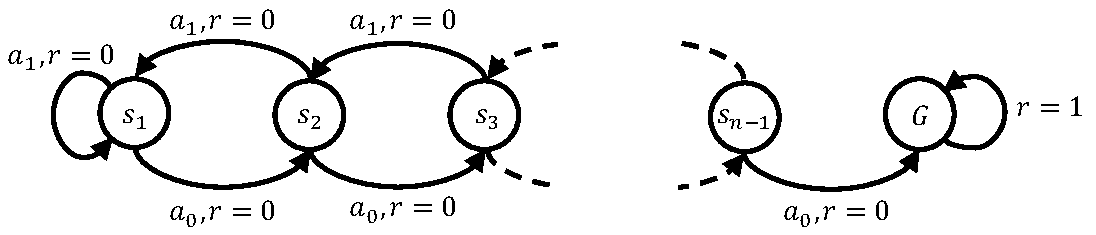
\includegraphics[width=0.7\textwidth]{mdp.pdf}
	\caption{$n$-state MDP}
	\label{fig:mdp}
\end{figure}

\subsection{Optimal action [5 points]}

What is the optimal policy, and does it depend on the value of the discount factor $\gamma$? Explain your answer.

{\color{blue}
	Your answer here.
}

\subsection{Optimal value function [10 points]}

Find the optimal value function for all states $s_i$ and the goal state $G$.
	
	{\color{blue}
		Your answer here.
	}
	
	
\subsection{Adding a constant to each reward [20 points]}
	
	Consider adding a constant $c$ to all rewards (i.e. taking any action from states $s_i$ has reward $c$ and any action from the goal state $G$ has reward $1+c$). Can adding a constant reward $c$ change the optimal policy? Derive the new optimal value function for all states $s_i$ and the goal state $G$.  Explain your answer.
	
	{\color{blue}
		Your answer here.
		
	}
	
\subsection{Scaling all the rewards by a constant [15 points]}	
	After adding a constant $c$ to all rewards now consider scaling all the rewards by a constant $a$ (i.e. $r_{new} = a(c+ r_{old})$). Can scaling rewards by $a$ change the optimal policy?
	Derive the new optimal value function for all states $s_i$ and the goal state $G$.
	
	{\color{blue}
		Your answer here.
	}


\section{Q-learning}
Consider the following Markov Decision Process.
It has two states $s$. It has two actions $a$: move and stay. The state transition is deterministic: ``move'' moves to the other state, while ``stay' stays at the current state. The reward $r$ is 0 for move,  1 for stay. There is a discounting factor $\gamma=0.8$.
\\

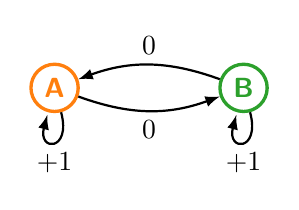
\begin{tikzpicture}
	\tikzstyle{n} = [very thick,circle,inner sep=0mm,minimum width=6mm]
	\tikzstyle{a} = [thick,>=latex,->]
	\def\dx{1.2}
	\def\dy{-1.2}
	\node[n,C1,draw=C1] (2) at (\dy,0) {\textbf{\textsf{A}}};
	\node[n,C2,draw=C2] (1) at (\dx,0) {\textbf{\textsf{B}}};
	\path[a]
	(2) edge [loop below] node {+1}(2)
	(1) edge [loop below] node {+1}(1)
	(2) edge [bend right=20] node[below] {0}(1)
	(1) edge [bend right=20] node[above] {0}(2);
\end{tikzpicture}

The reinforcement learning agent performs Q-learning.  Recall the $Q$ table has entries $Q(s,a)$. The $Q$ table is initialized with all zeros. The agent starts in state $s_1=A$. In any state $s_t$, the agent chooses the action $a_t$ according to a behavior policy $a_t = \pi_B(s_t)$. Upon experiencing the next state and reward $s_{t+1}, r_t$ the update is:
$$Q(s_t, a_t) \Leftarrow (1-\alpha) Q(s_t, a_t) + \alpha \left( r_t + \gamma \max_{a'} Q(s_{t+1}, a') \right).$$
Let the step size parameter $\alpha=0.5$.

\subsection{Greedy [15 points]}
	Run Q-learning for 200 steps with a deterministic greedy behavior policy: at each state $s_t$ use the best action $a_t \in \argmax_a Q(s_t,a)$ indicated by the current Q table. If there is a tie, prefer move. Show the Q table at the end.
	
	{\color{blue}
		Your answer here.
	}
	
\subsection{$\epsilon$-greedy [15 points]}

Reset and repeat the above, but with an $\epsilon$-greedy behavior policy: at each state $s_t$, with probability $1-\epsilon$ choose what the current Q table says is the best action: $\argmax_a Q(s_t,a)$; Break ties arbitrarily. Otherwise, (with probability $\epsilon$) uniformly chooses between move and stay (move or stay both with 1/2 probability). Use $\epsilon=0.5$.
	
	{\color{blue}
		Your answer here.
	}
	
\subsection{Bellman equation [20 points]}
	
	Without doing simulation, use Bellman equation to derive the true Q table induced by the MDP.
	
	{\color{blue}
		Your answer here.
		
	}
	

\end{document}
